% Options for packages loaded elsewhere
% Options for packages loaded elsewhere
\PassOptionsToPackage{unicode}{hyperref}
\PassOptionsToPackage{hyphens}{url}
%
\documentclass[
  ignorenonframetext,
  compress, aspectratio=149]{beamer}
\newif\ifbibliography
\usepackage{pgfpages}
\setbeamertemplate{caption}[numbered]
\setbeamertemplate{caption label separator}{: }
\setbeamercolor{caption name}{fg=normal text.fg}
\beamertemplatenavigationsymbolshorizontal
% remove section numbering
\setbeamertemplate{part page}{
  \centering
  \begin{beamercolorbox}[sep=16pt,center]{part title}
    \usebeamerfont{part title}\insertpart\par
  \end{beamercolorbox}
}
\setbeamertemplate{section page}{
  \centering
  \begin{beamercolorbox}[sep=12pt,center]{section title}
    \usebeamerfont{section title}\insertsection\par
  \end{beamercolorbox}
}
\setbeamertemplate{subsection page}{
  \centering
  \begin{beamercolorbox}[sep=8pt,center]{subsection title}
    \usebeamerfont{subsection title}\insertsubsection\par
  \end{beamercolorbox}
}
% Prevent slide breaks in the middle of a paragraph
\widowpenalties 1 10000
\raggedbottom
\AtBeginPart{
  \frame{\partpage}
}
\AtBeginSection{
  \ifbibliography
  \else
    \frame{\sectionpage}
  \fi
}
\AtBeginSubsection{
  \frame{\subsectionpage}
}
\usepackage{iftex}
\ifPDFTeX
  \usepackage[T1]{fontenc}
  \usepackage[utf8]{inputenc}
  \usepackage{textcomp} % provide euro and other symbols
\else % if luatex or xetex
  \usepackage{unicode-math} % this also loads fontspec
  \defaultfontfeatures{Scale=MatchLowercase}
  \defaultfontfeatures[\rmfamily]{Ligatures=TeX,Scale=1}
\fi
\usepackage{lmodern}

\usetheme[]{Montpellier}
\usecolortheme[]{dove}
\useinnertheme[]{rounded}
\useoutertheme[]{miniframes}
\ifPDFTeX\else
  % xetex/luatex font selection
\fi
% Use upquote if available, for straight quotes in verbatim environments
\IfFileExists{upquote.sty}{\usepackage{upquote}}{}
\IfFileExists{microtype.sty}{% use microtype if available
  \usepackage[]{microtype}
  \UseMicrotypeSet[protrusion]{basicmath} % disable protrusion for tt fonts
}{}
\makeatletter
\@ifundefined{KOMAClassName}{% if non-KOMA class
  \IfFileExists{parskip.sty}{%
    \usepackage{parskip}
  }{% else
    \setlength{\parindent}{0pt}
    \setlength{\parskip}{6pt plus 2pt minus 1pt}}
}{% if KOMA class
  \KOMAoptions{parskip=half}}
\makeatother

\usepackage{color}
\usepackage{fancyvrb}
\newcommand{\VerbBar}{|}
\newcommand{\VERB}{\Verb[commandchars=\\\{\}]}
\DefineVerbatimEnvironment{Highlighting}{Verbatim}{commandchars=\\\{\}}
% Add ',fontsize=\small' for more characters per line
\usepackage{framed}
\definecolor{shadecolor}{RGB}{248,248,248}
\newenvironment{Shaded}{\begin{snugshade}}{\end{snugshade}}
\newcommand{\AlertTok}[1]{\textcolor[rgb]{0.94,0.16,0.16}{#1}}
\newcommand{\AnnotationTok}[1]{\textcolor[rgb]{0.56,0.35,0.01}{\textbf{\textit{#1}}}}
\newcommand{\AttributeTok}[1]{\textcolor[rgb]{0.13,0.29,0.53}{#1}}
\newcommand{\BaseNTok}[1]{\textcolor[rgb]{0.00,0.00,0.81}{#1}}
\newcommand{\BuiltInTok}[1]{#1}
\newcommand{\CharTok}[1]{\textcolor[rgb]{0.31,0.60,0.02}{#1}}
\newcommand{\CommentTok}[1]{\textcolor[rgb]{0.56,0.35,0.01}{\textit{#1}}}
\newcommand{\CommentVarTok}[1]{\textcolor[rgb]{0.56,0.35,0.01}{\textbf{\textit{#1}}}}
\newcommand{\ConstantTok}[1]{\textcolor[rgb]{0.56,0.35,0.01}{#1}}
\newcommand{\ControlFlowTok}[1]{\textcolor[rgb]{0.13,0.29,0.53}{\textbf{#1}}}
\newcommand{\DataTypeTok}[1]{\textcolor[rgb]{0.13,0.29,0.53}{#1}}
\newcommand{\DecValTok}[1]{\textcolor[rgb]{0.00,0.00,0.81}{#1}}
\newcommand{\DocumentationTok}[1]{\textcolor[rgb]{0.56,0.35,0.01}{\textbf{\textit{#1}}}}
\newcommand{\ErrorTok}[1]{\textcolor[rgb]{0.64,0.00,0.00}{\textbf{#1}}}
\newcommand{\ExtensionTok}[1]{#1}
\newcommand{\FloatTok}[1]{\textcolor[rgb]{0.00,0.00,0.81}{#1}}
\newcommand{\FunctionTok}[1]{\textcolor[rgb]{0.13,0.29,0.53}{\textbf{#1}}}
\newcommand{\ImportTok}[1]{#1}
\newcommand{\InformationTok}[1]{\textcolor[rgb]{0.56,0.35,0.01}{\textbf{\textit{#1}}}}
\newcommand{\KeywordTok}[1]{\textcolor[rgb]{0.13,0.29,0.53}{\textbf{#1}}}
\newcommand{\NormalTok}[1]{#1}
\newcommand{\OperatorTok}[1]{\textcolor[rgb]{0.81,0.36,0.00}{\textbf{#1}}}
\newcommand{\OtherTok}[1]{\textcolor[rgb]{0.56,0.35,0.01}{#1}}
\newcommand{\PreprocessorTok}[1]{\textcolor[rgb]{0.56,0.35,0.01}{\textit{#1}}}
\newcommand{\RegionMarkerTok}[1]{#1}
\newcommand{\SpecialCharTok}[1]{\textcolor[rgb]{0.81,0.36,0.00}{\textbf{#1}}}
\newcommand{\SpecialStringTok}[1]{\textcolor[rgb]{0.31,0.60,0.02}{#1}}
\newcommand{\StringTok}[1]{\textcolor[rgb]{0.31,0.60,0.02}{#1}}
\newcommand{\VariableTok}[1]{\textcolor[rgb]{0.00,0.00,0.00}{#1}}
\newcommand{\VerbatimStringTok}[1]{\textcolor[rgb]{0.31,0.60,0.02}{#1}}
\newcommand{\WarningTok}[1]{\textcolor[rgb]{0.56,0.35,0.01}{\textbf{\textit{#1}}}}

\usepackage{longtable,booktabs,array}
\usepackage{calc} % for calculating minipage widths
\usepackage{caption}
% Make caption package work with longtable
\makeatletter
\def\fnum@table{\tablename~\thetable}
\makeatother
\usepackage{graphicx}
\makeatletter
\newsavebox\pandoc@box
\newcommand*\pandocbounded[1]{% scales image to fit in text height/width
  \sbox\pandoc@box{#1}%
  \Gscale@div\@tempa{\textheight}{\dimexpr\ht\pandoc@box+\dp\pandoc@box\relax}%
  \Gscale@div\@tempb{\linewidth}{\wd\pandoc@box}%
  \ifdim\@tempb\p@<\@tempa\p@\let\@tempa\@tempb\fi% select the smaller of both
  \ifdim\@tempa\p@<\p@\scalebox{\@tempa}{\usebox\pandoc@box}%
  \else\usebox{\pandoc@box}%
  \fi%
}
% Set default figure placement to htbp
\def\fps@figure{htbp}
\makeatother





\setlength{\emergencystretch}{3em} % prevent overfull lines

\providecommand{\tightlist}{%
  \setlength{\itemsep}{0pt}\setlength{\parskip}{0pt}}



 


\usepackage{booktabs}
\usepackage{longtable}
\usepackage{array}
\usepackage{multirow}
\usepackage{wrapfig}
\usepackage{float}
\usepackage{colortbl}
\usepackage{pdflscape}
\usepackage{tabu}
\usepackage{threeparttable}
\usepackage{threeparttablex}
\usepackage[normalem]{ulem}
\usepackage{makecell}
\usepackage{xcolor}
\usepackage{graphicx}
\usepackage{xcolor}
\usepackage{fancyvrb}
\usepackage{listings}
\definecolor{ColPrimario}{RGB}{100,8,58}
\definecolor{ColSecondario}{RGB}{20,143,184}
\setbeamercolor{structure}{fg=ColPrimario}
\setbeamercolor{itemize item}{fg=ColPrimario}
\setbeamercolor{itemize subitem}{fg=ColSecondario}
\setbeamercolor{palette primary}{bg=ColPrimario,fg=white}
\setbeamercolor{palette secondary}{bg=ColSecondario,fg=white}
\setbeamercolor{section in head/foot}{bg=ColPrimario,fg=white}
\setbeamercolor{subsection in head/foot}{bg=ColSecondario,fg=white}
\setbeamercolor{separation line}{fg=white}
\setbeamercolor{upper separation line head}{bg=white}
\setbeamercolor{middle separation line head}{bg=white}
\setbeamercolor{lower separation line head}{bg=white}

\lstset{basicstyle=\footnotesize\ttfamily, breaklines=true}

\DefineVerbatimEnvironment{Highlighting}{Verbatim}{commandchars=\\\{\}, fontsize=\footnotesize}
\DefineVerbatimEnvironment{verbatim}{Verbatim}{fontsize=\footnotesize}

\AtBeginSubsection{}

\AtBeginDocument{\institute[]{Università di Padova}}

\AtBeginDocument
{
  \author{Ottavia M. Epifania \\
  \texttt{ottavia.epifania@unipd.it} \\
  \textbf{Margherita Calderan} \\
  \texttt{margherita.calderan@unipd.it}}
  }

\AtBeginSection
{
  \begin{frame}[plain]
  \tableofcontents[currentsection, hideallsubsections]
  \end{frame}
  \begin{frame}[plain]
  \tableofcontents[currentsection,currentsubsection,hideothersubsections]
  \end{frame}
  }
\makeatletter
\@ifpackageloaded{caption}{}{\usepackage{caption}}
\AtBeginDocument{%
\ifdefined\contentsname
  \renewcommand*\contentsname{Table of contents}
\else
  \newcommand\contentsname{Table of contents}
\fi
\ifdefined\listfigurename
  \renewcommand*\listfigurename{List of Figures}
\else
  \newcommand\listfigurename{List of Figures}
\fi
\ifdefined\listtablename
  \renewcommand*\listtablename{List of Tables}
\else
  \newcommand\listtablename{List of Tables}
\fi
\ifdefined\figurename
  \renewcommand*\figurename{Figure}
\else
  \newcommand\figurename{Figure}
\fi
\ifdefined\tablename
  \renewcommand*\tablename{Table}
\else
  \newcommand\tablename{Table}
\fi
}
\@ifpackageloaded{float}{}{\usepackage{float}}
\floatstyle{ruled}
\@ifundefined{c@chapter}{\newfloat{codelisting}{h}{lop}}{\newfloat{codelisting}{h}{lop}[chapter]}
\floatname{codelisting}{Listing}
\newcommand*\listoflistings{\listof{codelisting}{List of Listings}}
\makeatother
\makeatletter
\makeatother
\makeatletter
\@ifpackageloaded{caption}{}{\usepackage{caption}}
\@ifpackageloaded{subcaption}{}{\usepackage{subcaption}}
\makeatother

\usepackage{bookmark}
\IfFileExists{xurl.sty}{\usepackage{xurl}}{} % add URL line breaks if available
\urlstyle{same}
\hypersetup{
  pdftitle={Frequenze e Indici di Tendenza Centrale},
  pdfauthor={Ottavia M. Epifania, Margherita Calderan},
  hidelinks,
  pdfcreator={LaTeX via pandoc}}


\title{Frequenze e Indici di Tendenza Centrale}
\subtitle{Test per le organizzaioni}
\author{Ottavia M. Epifania, Margherita Calderan}
\date{02/2026}

\begin{document}
\frame{\titlepage}


\section{Statistica descrittiva e
inferenziale}\label{statistica-descrittiva-e-inferenziale}

\begin{frame}{Statistica descrittiva e inferenziale}
\begin{itemize}
\tightlist
\item
  \textbf{Statistica descrittiva}

  \begin{itemize}
  \tightlist
  \item
    Riassume, descrive, esplora i dati osservati\\
  \item
    Prima fase nella valutazione delle proprietà psicometriche di uno
    strumento
  \end{itemize}
\item
  \textbf{Statistica inferenziale}

  \begin{itemize}
  \tightlist
  \item
    Usa i dati di un \textbf{campione} per fare inferenze sulla
    \textbf{popolazione}\\
  \item
    Confronti tra gruppi, valutazione di interventi, validazione di test
  \end{itemize}
\end{itemize}
\end{frame}

\subsection{La statistica descrittiva}\label{la-statistica-descrittiva}

\begin{frame}{La statistica descrittiva}
\begin{itemize}
\item
  È utile per controllare, descrivere ed esplorare i dati
\item
  Serve a riassumere i dati attraverso indici statistici, tabelle e
  grafici
\item
  \textbf{Non esiste una buona analisi statistica, senza una buona
  analisi descrittiva}
\end{itemize}
\end{frame}

\subsection{Tecniche}\label{tecniche}

\begin{frame}{Tecniche}
\begin{itemize}
\item
  \textbf{Distribuzione di frequenza e grafici}
\item
  \textbf{Indici di tendenza centrale/indici di posizione}
\item
  \textbf{Indici di variabilità}
\end{itemize}
\end{frame}

\section{Dati}\label{dati}

\begin{frame}[fragile]{Dati}
Il dataset sintetico contiene dati individuali relativi a dipendenti di
un'azienda e viene utilizzato per modellare il rischio di burnout e
analizzare i fattori associati al benessere lavorativo. Come prima cosa
vogliamo esplorare la distribuzione di livelli di stess (variabile
\texttt{StressLevel})

\href{https://www.kaggle.com/datasets/ankam6010/synthetic-hr-burnout-dataset/data}{fonte
dati}
\end{frame}

\begin{frame}[fragile]
Carichiamo il dataset:

\begin{Shaded}
\begin{Highlighting}[]
\CommentTok{\# installo pacchetti, vedi script pkg.R}

\CommentTok{\# carico pacchetti}
\FunctionTok{library}\NormalTok{(dplyr)}
\FunctionTok{library}\NormalTok{(readr)}

\CommentTok{\# carico dataset}
\NormalTok{burnout }\OtherTok{=} \FunctionTok{read\_csv}\NormalTok{(}\StringTok{"data/burnout.csv"}\NormalTok{)}
\end{Highlighting}
\end{Shaded}
\end{frame}

\begin{frame}[fragile]
Visualizzo la struttura:

\begin{Shaded}
\begin{Highlighting}[]
\FunctionTok{str}\NormalTok{(burnout)}
\end{Highlighting}
\end{Shaded}

\begin{verbatim}
spc_tbl_ [2,000 x 10] (S3: spec_tbl_df/tbl_df/tbl/data.frame)
 $ Name             : chr [1:2000] "Max Ivanov" "Max Wang" "Nina Petrov" "John Ivanov" ...
 $ Age              : num [1:2000] 32 40 33 35 59 45 31 39 24 22 ...
 $ Gender           : chr [1:2000] "Male" "Female" "Female" "Female" ...
 $ JobRole          : chr [1:2000] "Analyst" "Engineer" "Engineer" "Manager" ...
 $ Experience       : num [1:2000] 3 9 2 6 8 11 5 17 0 1 ...
 $ WorkHoursPerWeek : num [1:2000] 60 47 44 44 38 44 70 31 63 30 ...
 $ RemoteRatio      : num [1:2000] 21 67 20 70 46 90 30 53 35 5 ...
 $ SatisfactionLevel: num [1:2000] 4.4 2.09 2.58 3.23 4.41 4.31 2.18 3.95 1.32 1.44 ...
 $ StressLevel      : num [1:2000] 1 2 3 8 1 7 3 4 5 5 ...
 $ Burnout          : num [1:2000] 0 0 0 0 0 0 0 0 0 0 ...
 - attr(*, "spec")=
  .. cols(
  ..   Name = col_character(),
  ..   Age = col_double(),
  ..   Gender = col_character(),
  ..   JobRole = col_character(),
  ..   Experience = col_double(),
  ..   WorkHoursPerWeek = col_double(),
  ..   RemoteRatio = col_double(),
  ..   SatisfactionLevel = col_double(),
  ..   StressLevel = col_double(),
  ..   Burnout = col_double()
  .. )
 - attr(*, "problems")=<externalptr> 
\end{verbatim}
\end{frame}

\begin{frame}[fragile]
Sebbene \texttt{StressLevel} sia una variabile quantitativa discreta su
scala 1--10, il manager dell'azienda ha richiesto di descriverla
assumendola variabile categoriale ordinale.

\begin{Shaded}
\begin{Highlighting}[]
\FunctionTok{str}\NormalTok{(burnout}\SpecialCharTok{$}\NormalTok{StressLevel)}
\end{Highlighting}
\end{Shaded}

\begin{verbatim}
 num [1:2000] 1 2 3 8 1 7 3 4 5 5 ...
\end{verbatim}
\end{frame}

\begin{frame}[fragile]
In particolare, i livelli di stress sono stati categorizzati in tre
fasce: \textbf{basso} (1--2), \textbf{moderato} (3--4), \textbf{alto}
(5--7), e \textbf{severo} (8--10). A tale scopo, creiamo una nuova
variabile che rappresenta una versione categorizzata di
\texttt{StressLevel}.

\begin{Shaded}
\begin{Highlighting}[]
\CommentTok{\# creo la variabile StressLevel}
\NormalTok{StressCat }\OtherTok{=} \FunctionTok{case\_when}\NormalTok{(}
\NormalTok{  burnout}\SpecialCharTok{$}\NormalTok{StressLevel }\SpecialCharTok{\textless{}=} \DecValTok{2} \SpecialCharTok{\textasciitilde{}} \StringTok{"basso"}\NormalTok{, }
\NormalTok{  burnout}\SpecialCharTok{$}\NormalTok{StressLevel  }\SpecialCharTok{\textgreater{}=} \DecValTok{3} \SpecialCharTok{\&}\NormalTok{ burnout}\SpecialCharTok{$}\NormalTok{StressLevel  }\SpecialCharTok{\textless{}=} \DecValTok{4} \SpecialCharTok{\textasciitilde{}} \StringTok{"moderato"}\NormalTok{,}
\NormalTok{  burnout}\SpecialCharTok{$}\NormalTok{StressLevel  }\SpecialCharTok{\textgreater{}=} \DecValTok{5} \SpecialCharTok{\&}\NormalTok{ burnout}\SpecialCharTok{$}\NormalTok{StressLevel  }\SpecialCharTok{\textless{}=} \DecValTok{7} \SpecialCharTok{\textasciitilde{}} \StringTok{"alto"}\NormalTok{,}
\NormalTok{  burnout}\SpecialCharTok{$}\NormalTok{StressLevel  }\SpecialCharTok{\textgreater{}=} \DecValTok{8} \SpecialCharTok{\textasciitilde{}} \StringTok{"severo"}\NormalTok{ )}

\FunctionTok{str}\NormalTok{(StressCat)}
\end{Highlighting}
\end{Shaded}

\begin{verbatim}
 chr [1:2000] "basso" "basso" "moderato" "severo" "basso" "alto" "moderato" ...
\end{verbatim}
\end{frame}

\begin{frame}[fragile]
Così come esiste il comando \texttt{factor}, possiamo utilizzare il
comando \texttt{ordered} per definire una variabile categoriale
ordinale.

\begin{Shaded}
\begin{Highlighting}[]
\NormalTok{StressCat }\OtherTok{=} \FunctionTok{ordered}\NormalTok{(StressCat, }
           \AttributeTok{levels=}\FunctionTok{c}\NormalTok{(}\StringTok{"basso"}\NormalTok{,}\StringTok{"moderato"}\NormalTok{,}\StringTok{"alto"}\NormalTok{,}\StringTok{"severo"}\NormalTok{))}
\CommentTok{\# attraverso l\textquotesingle{}argomento levels specifichiamo l\textquotesingle{}ORDINE dei livelli/categorie}
\FunctionTok{str}\NormalTok{(StressCat)}
\end{Highlighting}
\end{Shaded}

\begin{verbatim}
 Ord.factor w/ 4 levels "basso"<"moderato"<..: 1 1 2 4 1 3 2 2 3 3 ...
\end{verbatim}

\begin{Shaded}
\begin{Highlighting}[]
\CommentTok{\#Aggiugo la nuova variabile al dataset}
\NormalTok{burnout}\SpecialCharTok{$}\NormalTok{StressCat }\OtherTok{=}\NormalTok{ StressCat}
\end{Highlighting}
\end{Shaded}
\end{frame}

\section{Frequenze}\label{frequenze}

\subsection{Notazioni fondamentali}\label{notazioni-fondamentali}

\begin{frame}[fragile]{Notazioni fondamentali}
\begin{itemize}
\item
  Sia \(X\) la variabile \texttt{StressCat}
\item
  Sia \(Xi\) la categoria/livello \(i\)−esima di \(X\), dove
  \(i = 1 \dots 4\)
\item
  Sia \(n\) il totale delle unità statistiche (\(n = 2000\))
\end{itemize}
\end{frame}

\subsection{Le frequenze assolute
semplici}\label{le-frequenze-assolute-semplici}

\begin{frame}[fragile]{Le frequenze assolute semplici}
La frequenza assoluta semplice di una categoria è il \textbf{numero
naturale di unità statistiche} che presentano tale categoria.

Se vogliamo calcolare le frequenze assolute semplici per ogni
categoria/livello, possiamo utilizzare la funzione \texttt{table()}

\begin{Shaded}
\begin{Highlighting}[]
\FunctionTok{table}\NormalTok{(burnout}\SpecialCharTok{$}\NormalTok{StressCat) }\CommentTok{\# nome\_dataframe$nome\_variabile}
\end{Highlighting}
\end{Shaded}

\begin{verbatim}

   basso moderato     alto   severo 
     419      399      584      598 
\end{verbatim}
\end{frame}

\subsection{Le frequenze assolute
cumulate}\label{le-frequenze-assolute-cumulate}

\begin{frame}[fragile]{Le frequenze assolute cumulate}
La frequenza assoluta cumulata di una categoria/livello è la
\textbf{somma} delle \textbf{frequenze assolute semplici} delle
categorie precedenti alla categoria data più la frequenza assoluta
semplice della categoria data.

Attraverso la funzione \texttt{cumsum()} possiamo calcolare la somma
cumulata, in questo caso le frequenze assolute cumulate

\begin{Shaded}
\begin{Highlighting}[]
\FunctionTok{table}\NormalTok{(burnout}\SpecialCharTok{$}\NormalTok{StressCat)}
\end{Highlighting}
\end{Shaded}

\begin{verbatim}

   basso moderato     alto   severo 
     419      399      584      598 
\end{verbatim}

\begin{Shaded}
\begin{Highlighting}[]
\FunctionTok{cumsum}\NormalTok{(}\FunctionTok{table}\NormalTok{(burnout}\SpecialCharTok{$}\NormalTok{StressCat))}
\end{Highlighting}
\end{Shaded}

\begin{verbatim}
   basso moderato     alto   severo 
     419      818     1402     2000 
\end{verbatim}
\end{frame}

\subsection{Le frequenze relative
semplici}\label{le-frequenze-relative-semplici}

\begin{frame}[fragile]{Le frequenze relative semplici}
La frequenza relativa semplice è data dal rapporto tra la
\textbf{frequenza assoluta semplice di tale categoria} e \textbf{il
numero totale} di unità statistiche osservate

Qual'è il numero totale di unità statistiche?

\begin{Shaded}
\begin{Highlighting}[]
\FunctionTok{nrow}\NormalTok{(burnout) }\CommentTok{\#numero righe dataframe}
\end{Highlighting}
\end{Shaded}

\begin{verbatim}
[1] 2000
\end{verbatim}

\begin{Shaded}
\begin{Highlighting}[]
\FunctionTok{length}\NormalTok{(burnout}\SpecialCharTok{$}\NormalTok{StressCat) }\CommentTok{\# lunghezza della variabile }
\end{Highlighting}
\end{Shaded}

\begin{verbatim}
[1] 2000
\end{verbatim}

\begin{Shaded}
\begin{Highlighting}[]
\NormalTok{n }\OtherTok{=} \FunctionTok{nrow}\NormalTok{(burnout) }\CommentTok{\#oggetto n = numero unità stat}
\end{Highlighting}
\end{Shaded}
\end{frame}

\begin{frame}[fragile]
Qual'è frequenza relativa semplice associata alle categorie/livelli?

\begin{Shaded}
\begin{Highlighting}[]
\FunctionTok{table}\NormalTok{(burnout}\SpecialCharTok{$}\NormalTok{StressCat)}\SpecialCharTok{/}\NormalTok{n}
\end{Highlighting}
\end{Shaded}

\begin{verbatim}

   basso moderato     alto   severo 
  0.2095   0.1995   0.2920   0.2990 
\end{verbatim}

\textbf{Una frequenza relativa semplice varia sempre tra 0 e 1.}
\end{frame}

\subsection{Le frequenze relative
cumulate}\label{le-frequenze-relative-cumulate}

\begin{frame}[fragile]{Le frequenze relative cumulate}
La frequenza relativa cumulata di una categoria è la \textbf{somma delle
frequenze relative semplice} delle categorie precedenti alla categoria
data più la frequenza relativa semplice della categoria data.

Come prima, attraverso la funzione \texttt{cumsum()}, possiamo calcolare
le frequenze relative \textbf{cumulate}

\begin{Shaded}
\begin{Highlighting}[]
\FunctionTok{cumsum}\NormalTok{(}\FunctionTok{table}\NormalTok{(burnout}\SpecialCharTok{$}\NormalTok{StressCat)}\SpecialCharTok{/}\NormalTok{n)}
\end{Highlighting}
\end{Shaded}

\begin{verbatim}
   basso moderato     alto   severo 
  0.2095   0.4090   0.7010   1.0000 
\end{verbatim}

Ad esempio, \(P_2 = 0.409\), indica che \textasciitilde40\% rispondenti
ha riportato un grado di stress inferiore o uguale a moderato.

\textbf{Una frequenza relativa cumulata varia sempre tra 0 e 1.}
\end{frame}

\begin{frame}
\begin{longtable}[]{@{}ccccccc@{}}
\toprule\noalign{}
Indice i & Categoria & Xi & fi & Fi & pi & Pi \\
\midrule\noalign{}
\endhead
1 & basso & 1 & 419 & 419 & 0.2095 & 0.2095 \\
2 & moderato & 2 & 399 & 818 & 0.1995 & 0.4090 \\
3 & alto & 3 & 584 & 1402 & 0.2920 & 0.7010 \\
4 & severo & 4 & 598 & 2000 & 0.2990 & 1.0000 \\
\bottomrule\noalign{}
\end{longtable}
\end{frame}

\subsection{Visualizzazione}\label{visualizzazione}

\begin{frame}[fragile]
\begin{Shaded}
\begin{Highlighting}[]
\FunctionTok{barplot}\NormalTok{(}\FunctionTok{table}\NormalTok{(burnout}\SpecialCharTok{$}\NormalTok{StressCat), }\AttributeTok{ylab=}\StringTok{"?"}\NormalTok{, }
         \AttributeTok{xlab=}\StringTok{" "}\NormalTok{,}\AttributeTok{ylim =}\FunctionTok{c}\NormalTok{(}\DecValTok{0}\NormalTok{,}\DecValTok{600}\NormalTok{)) }\CommentTok{\# diagramma a barre}
\end{Highlighting}
\end{Shaded}

\pandocbounded{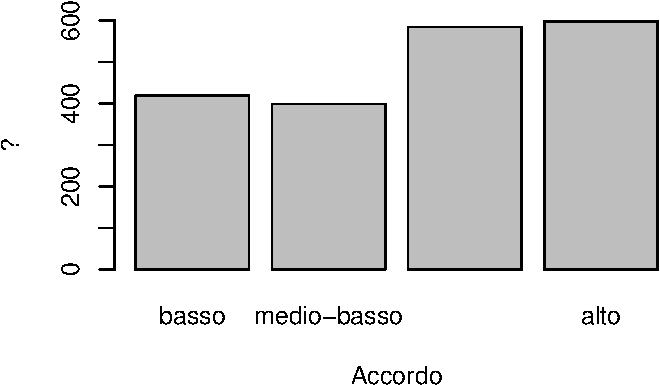
\includegraphics[keepaspectratio]{0-Descrittiva_files/figure-beamer/unnamed-chunk-12-1.pdf}}
\end{frame}

\begin{frame}[fragile]
\begin{Shaded}
\begin{Highlighting}[]
\FunctionTok{barplot}\NormalTok{(}\FunctionTok{table}\NormalTok{(burnout}\SpecialCharTok{$}\NormalTok{StressCat)}\SpecialCharTok{/}\NormalTok{n, }\AttributeTok{ylab=}\StringTok{"?"}\NormalTok{, }
         \AttributeTok{xlab=}\StringTok{" "}\NormalTok{, }\AttributeTok{ylim =}\FunctionTok{c}\NormalTok{(}\DecValTok{0}\NormalTok{,.}\DecValTok{3}\NormalTok{)) }\CommentTok{\# diagramma a barre}
\end{Highlighting}
\end{Shaded}

\pandocbounded{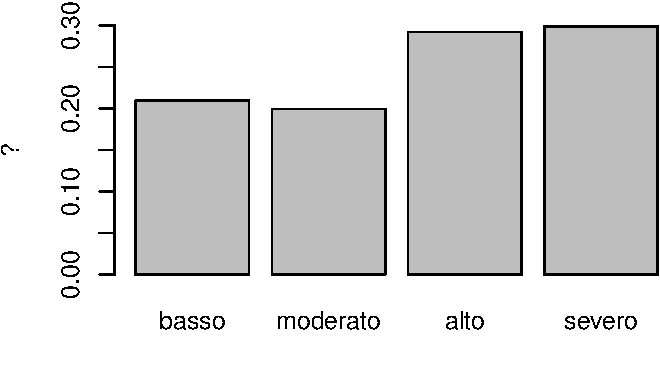
\includegraphics[keepaspectratio]{0-Descrittiva_files/figure-beamer/unnamed-chunk-13-1.pdf}}
\end{frame}

\begin{frame}[fragile]
\begin{Shaded}
\begin{Highlighting}[]
\FunctionTok{barplot}\NormalTok{(}\FunctionTok{cumsum}\NormalTok{(}\FunctionTok{table}\NormalTok{(burnout}\SpecialCharTok{$}\NormalTok{StressCat)), }\AttributeTok{ylab=}\StringTok{"?"}\NormalTok{, }
         \AttributeTok{xlab=}\StringTok{" "}\NormalTok{) }\CommentTok{\# diagramma a barre}
\end{Highlighting}
\end{Shaded}

\pandocbounded{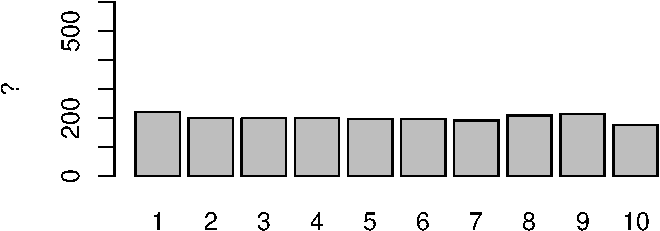
\includegraphics[keepaspectratio]{0-Descrittiva_files/figure-beamer/unnamed-chunk-14-1.pdf}}
\end{frame}

\begin{frame}[fragile]
\begin{Shaded}
\begin{Highlighting}[]
\FunctionTok{barplot}\NormalTok{(}\FunctionTok{cumsum}\NormalTok{(}\FunctionTok{table}\NormalTok{(burnout}\SpecialCharTok{$}\NormalTok{StressCat))}\SpecialCharTok{/}\NormalTok{n, }\AttributeTok{ylab=}\StringTok{"?"}\NormalTok{, }
         \AttributeTok{xlab=}\StringTok{" "}\NormalTok{) }\CommentTok{\# diagramma a barre}
\end{Highlighting}
\end{Shaded}

\pandocbounded{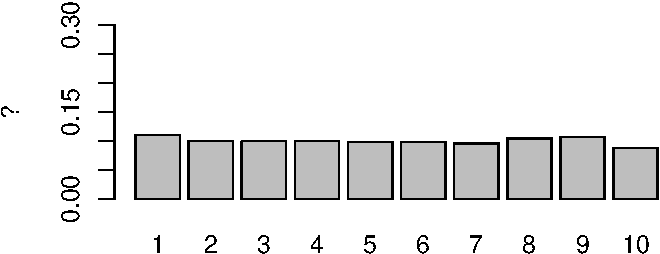
\includegraphics[keepaspectratio]{0-Descrittiva_files/figure-beamer/unnamed-chunk-15-1.pdf}}
\end{frame}

\section{Indici di tendenza centrale}\label{indici-di-tendenza-centrale}

\begin{frame}{Indici di tendenza centrale}
Un indice di tendenza centrale è un valore che descrive e riassume il
centro di una distribuzione di dati.

\begin{tabular}{lccc}
\toprule
Indice & Variabile nominale & Variabile ordinale & Variabile quantitativa\\
\midrule
Moda & SI & SI & SI\\
Mediana & NO & SI & SI\\
Media & NO & NO & SI\\
\bottomrule
\end{tabular}
\end{frame}

\subsection{La moda}\label{la-moda}

\begin{frame}[fragile]{La moda}
La moda di una distribuzione di dati rilevati sulla variabile \(X\), è
la categoria che si presenta con la massima frequenza.

Ad esempio, rispetto ai dati relativi ai livelli di stress, la moda è
\ldots.

\begin{verbatim}

   basso moderato     alto   severo 
     419      399      584      598 
\end{verbatim}
\end{frame}

\begin{frame}[fragile]
Che funzione posso usare per ottenere la moda?

\begin{Shaded}
\begin{Highlighting}[]
\FunctionTok{table}\NormalTok{(burnout}\SpecialCharTok{$}\NormalTok{StressCat)}
\end{Highlighting}
\end{Shaded}

\begin{verbatim}

   basso moderato     alto   severo 
     419      399      584      598 
\end{verbatim}
\end{frame}

\subsection{La mediana}\label{la-mediana}

\begin{frame}{La mediana}
\begin{itemize}
\tightlist
\item
  La mediana di una distribuzione di dati ordinati rilevati sulla
  variabile \(X\), è il dato che occupa la posizione centrale rispetto
  alla distribuzione dei dati.
\end{itemize}
\end{frame}

\begin{frame}[fragile]{Calcolo della mediana}
\phantomsection\label{calcolo-della-mediana}
Si individua la prima frequenza cumulata maggiore o uguale della
posizione cercata:

\begin{Shaded}
\begin{Highlighting}[]
\NormalTok{n }\OtherTok{=} \FunctionTok{nrow}\NormalTok{(burnout); n}
\end{Highlighting}
\end{Shaded}

\begin{verbatim}
[1] 2000
\end{verbatim}

\begin{Shaded}
\begin{Highlighting}[]
\CommentTok{\# Qual\textquotesingle{}è la posizione centrale?}
\NormalTok{i }\OtherTok{=}\NormalTok{ (n}\SpecialCharTok{+}\DecValTok{1}\NormalTok{)}\SpecialCharTok{/}\DecValTok{2}
\NormalTok{i}
\end{Highlighting}
\end{Shaded}

\begin{verbatim}
[1] 1000.5
\end{verbatim}

\begin{Shaded}
\begin{Highlighting}[]
\CommentTok{\# calcolo frequenza cumulata}
\FunctionTok{cumsum}\NormalTok{(}\FunctionTok{table}\NormalTok{(burnout}\SpecialCharTok{$}\NormalTok{StressCat))}
\end{Highlighting}
\end{Shaded}

\begin{verbatim}
   basso moderato     alto   severo 
     419      818     1402     2000 
\end{verbatim}
\end{frame}

\begin{frame}[fragile]{Calcolo della mediana}
\phantomsection\label{calcolo-della-mediana-1}
Attraverso la funzione \texttt{sort} si possono riordinare gli elementi
di un vettore (nel nostro caso la variabile \texttt{StressCat})

\begin{Shaded}
\begin{Highlighting}[]
\NormalTok{StressCatOrd }\OtherTok{=} \FunctionTok{sort}\NormalTok{(burnout}\SpecialCharTok{$}\NormalTok{StressCat)}

\CommentTok{\# visualizzo i primi elementi variabile ordinata}
\FunctionTok{head}\NormalTok{(StressCatOrd, }\AttributeTok{n =} \DecValTok{6}\NormalTok{)}
\end{Highlighting}
\end{Shaded}

\begin{verbatim}
[1] basso basso basso basso basso basso
Levels: basso < moderato < alto < severo
\end{verbatim}

\begin{Shaded}
\begin{Highlighting}[]
\CommentTok{\# prima}
\FunctionTok{head}\NormalTok{(burnout}\SpecialCharTok{$}\NormalTok{StressCat, }\AttributeTok{n =} \DecValTok{6}\NormalTok{)}
\end{Highlighting}
\end{Shaded}

\begin{verbatim}
[1] basso    basso    moderato severo   basso    alto    
Levels: basso < moderato < alto < severo
\end{verbatim}
\end{frame}

\begin{frame}[fragile]{Calcolo della mediana: caso n pari}
\phantomsection\label{calcolo-della-mediana-caso-n-pari}
Nel caso di \emph{n} dispari, la mediana sarà semplicemente il valore
che sta al centro. Nel caso invece di \emph{n} pari, possiamo trovare le
posizioni tra cui si trova la mediana:

\begin{itemize}
\tightlist
\item
  inferiore \(\frac{n}{2}\)
\item
  superiore \(\frac{n}{2} + 1\)
\end{itemize}

\begin{Shaded}
\begin{Highlighting}[]
\NormalTok{StressCatOrd[n}\SpecialCharTok{/}\DecValTok{2}\NormalTok{] }\CommentTok{\# i\_inf = n/2}
\end{Highlighting}
\end{Shaded}

\begin{verbatim}
[1] alto
Levels: basso < moderato < alto < severo
\end{verbatim}

\begin{Shaded}
\begin{Highlighting}[]
\NormalTok{StressCatOrd[(n}\SpecialCharTok{/}\DecValTok{2}\NormalTok{) }\SpecialCharTok{+} \DecValTok{1}\NormalTok{] }\CommentTok{\# i\_sup = (n/2) + 1}
\end{Highlighting}
\end{Shaded}

\begin{verbatim}
[1] alto
Levels: basso < moderato < alto < severo
\end{verbatim}
\end{frame}

\subsection{La media aritmetica}\label{la-media-aritmetica}

\begin{frame}[fragile]{La media aritmetica}
La media aritmetica di una distribuzione di dati rilevati sulla
variabile \(X\), è data dalla somma dei dati divisa per il numero di
unità statistiche.

In questo caso possiamo calcolare la media dei livelli di Stress in
quanto variabile quantitativa:

\begin{Shaded}
\begin{Highlighting}[]
\FunctionTok{str}\NormalTok{(burnout}\SpecialCharTok{$}\NormalTok{StressLevel)}
\end{Highlighting}
\end{Shaded}

\begin{verbatim}
 num [1:2000] 1 2 3 8 1 7 3 4 5 5 ...
\end{verbatim}
\end{frame}

\begin{frame}[fragile]
Calcolo della media :

\begin{Shaded}
\begin{Highlighting}[]
\CommentTok{\# numero di unità}
\NormalTok{n }\OtherTok{=} \FunctionTok{length}\NormalTok{(burnout}\SpecialCharTok{$}\NormalTok{StressLevel) }

\CommentTok{\# sommo tutti gli elementi e divido per n}
\FunctionTok{sum}\NormalTok{(burnout}\SpecialCharTok{$}\NormalTok{StressLevel)}\SpecialCharTok{/}\NormalTok{n }
\end{Highlighting}
\end{Shaded}

\begin{verbatim}
[1] 5.432
\end{verbatim}

\begin{Shaded}
\begin{Highlighting}[]
\CommentTok{\# funzione mean}
\FunctionTok{mean}\NormalTok{(burnout}\SpecialCharTok{$}\NormalTok{StressLevel)}
\end{Highlighting}
\end{Shaded}

\begin{verbatim}
[1] 5.432
\end{verbatim}
\end{frame}

\section{Credits}\label{credits}

\begin{frame}{Credits}
Altoè, G. (2022). Corso di Testing Psicologico, Scienze psicologiche
dello sviluppo, della personalità e delle relazioni interpersonali, A.A.
2022/23

Marci, M. (2025). Corso di Testing Psicologico, Scienze psicologiche
dello sviluppo, della personalità e delle relazioni interpersonali, A.A.
2025/26

\href{https://www.kaggle.com/datasets/ankam6010/synthetic-hr-burnout-dataset/data}{Fonte
dati}
\end{frame}




\end{document}
